\documentclass[11pt, margin=1in]{article}
\usepackage{fancyhdr}
\usepackage[margin=1in]{geometry}
\usepackage{graphicx}
\usepackage{hyperref}
\usepackage{amsmath}
\graphicspath{ {images/} }

\pagestyle{fancy}
\lhead{\textbf{sm@rticle} - the smart article summarizer}
\rhead{\textit{Alex Lin (alexanderlin01@college.harvard.edu)}}
\cfoot{\thepage}
\renewcommand{\headrulewidth}{0.4pt}
\renewcommand{\footrulewidth}{0.4pt}
\makeatletter

\newcommand{\card}[1]{\ensuremath{\left\vert#1\right\vert}}

\begin{document}

\title{\textbf{sm@rticle}}
\author{\textit{Alex Lin}}
\date{April 3, 2016}
\maketitle

%%%%OVERVIEW%%%%
\noindent 
\textbf{Overview:} sm@rticle is a Swift-based iPhone application developed by Alex Lin that smartly generates short summaries of news articles.  It mainly utilizes an unsupervised machine-learning algorithm similar to Google's PageRank.  

%%%%INSTRUCTIONS%%%%

\section{Setup Instructions}
\begin{enumerate}

\item
Pull the sm@rticle repository from the following link: https://github.com/al5250/smarticle.  You should find the following files:
\begin{center}
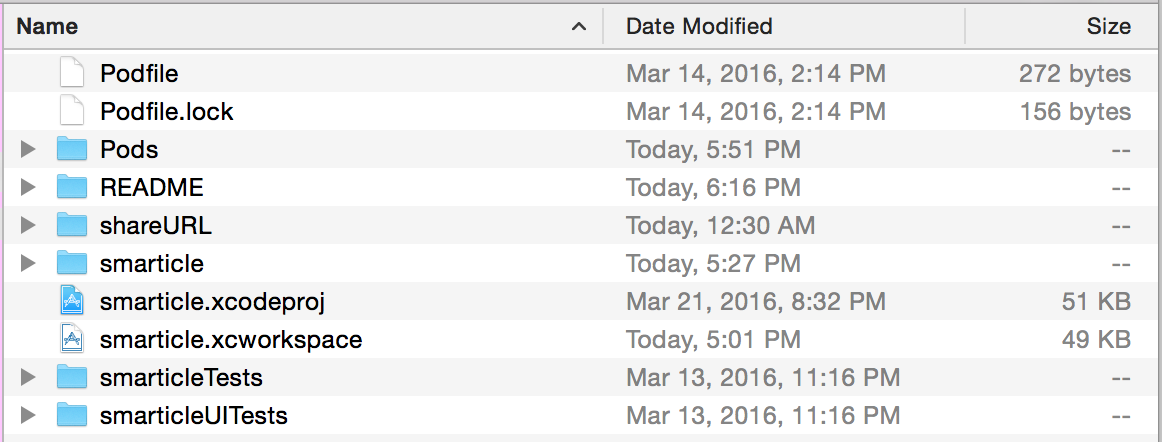
\includegraphics[scale=0.7]{1.jpg}
\end{center}

\item
Open the file "smarticle.xcworkspace" with Xcode.  Make sure the application is set to "smarticle" in the top left corner.  Run the project with the big "Play" button.     
\begin{center}
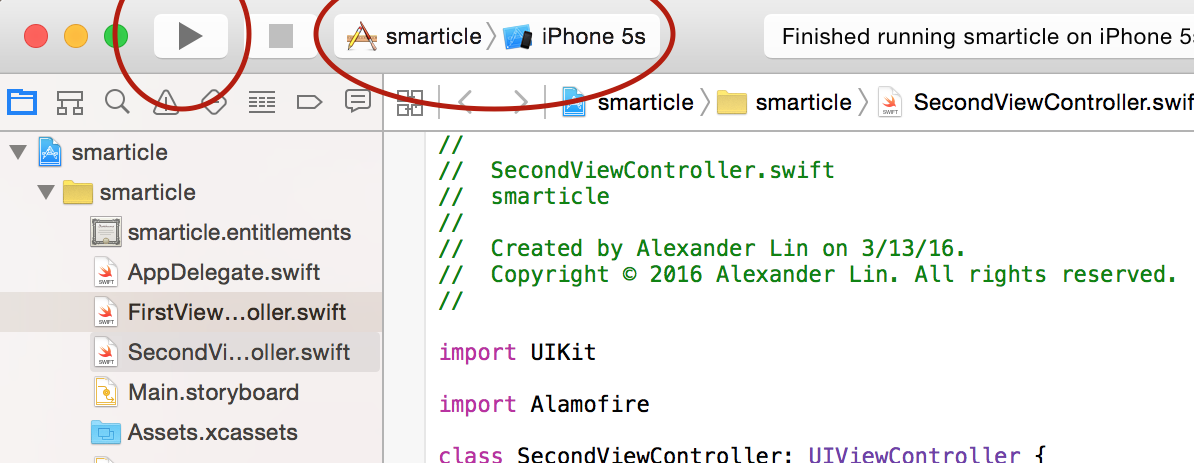
\includegraphics[scale=0.7]{2.jpg}
\end{center}

\item
The application will now load.  Notice that there are two main functions - "Search" and "Browse".  "Search" will be the default tab selected.  
\begin{center}
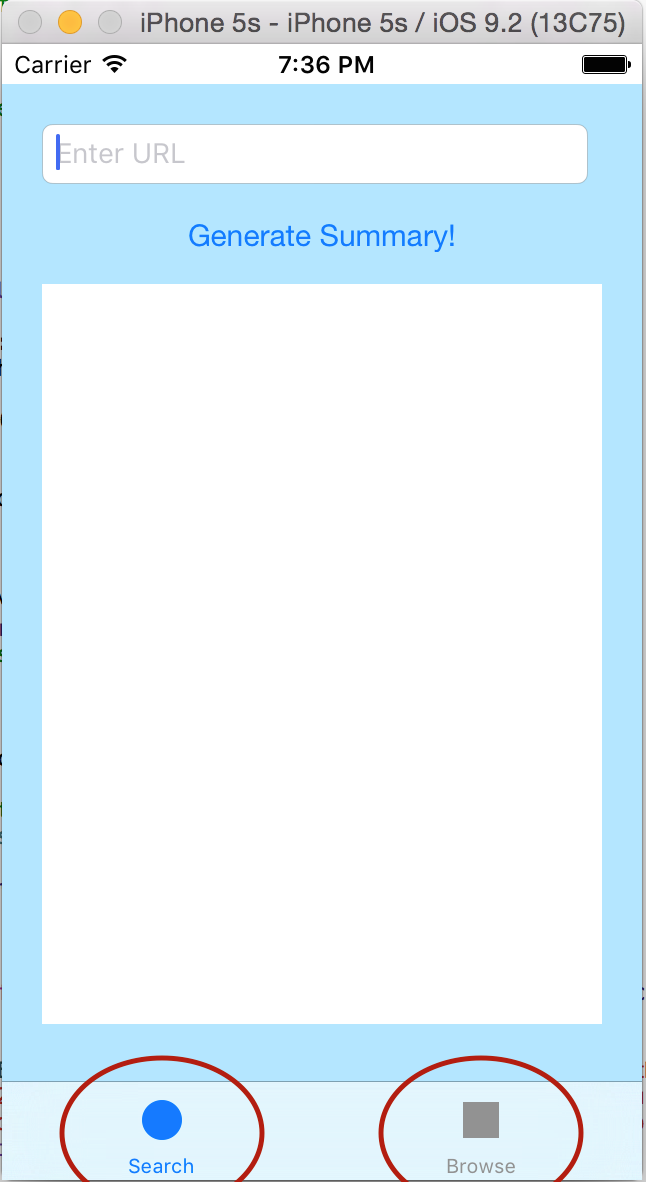
\includegraphics[scale=0.7]{3.jpg}
\end{center}

\end{enumerate}

\newpage

%%%%FEATURES%%%%

\section{Main Features and Functions}

There are three main components of sm@rticle - 1) "Search", which generates summaries for specific articles; 2) "Browse", which allows you to search for articles by keyword, and 3) "ShareURL", which is a share extension that allows you to pass in an article's URL from a web browser such as Safari.  

\subsection{Search}
"Search" works in a very self-explanatory fashion.  Simply enter a URL in the indicated text box and hit the "Generate Summary!" button.  If you enter in a valid URL, then the app will construct a summary of the article consisting of four sentences and display the title and this summary in the text field below.  Here is an example: 
\begin{center}
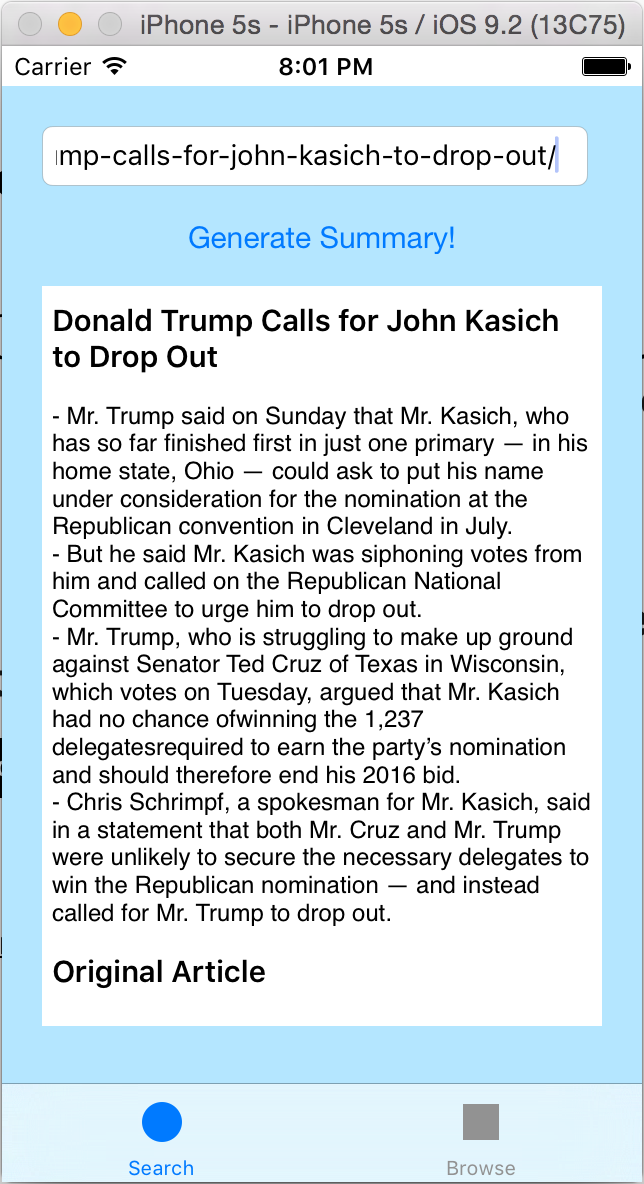
\includegraphics[scale=0.7]{4.jpg}
\end{center}
If you want to read the original article, simply scroll down and you will find the exact wording of the website.  Conversely, if the text you entered in the text box is not a valid URL, then you will be prompted with the following message:    
\begin{center}

\includegraphics[scale=0.7]{5.jpg}
\end{center}

\subsection{Browse}
"Browse" is the second tab of sm@rticle, and it allows you to browse for articles by their title.  I implemented "Browse" as an additional bonus objective. 
Simply enter in a key word or phrase into the textbox, and hit the button "Find Articles!"  The names of up to 8 articles will appear as buttons on the screen.  
\begin{center}
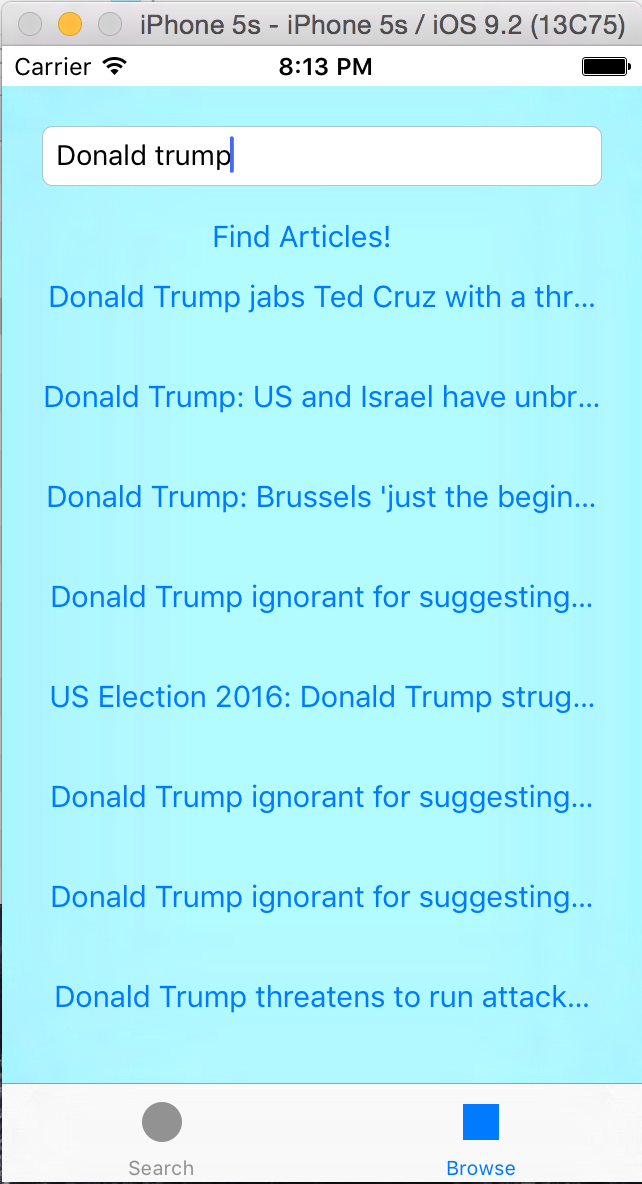
\includegraphics[scale=0.7]{6.jpg}
\end{center}
Click on any one of these buttons and you will be automatically redirected to "Search", with the URL for the corresponding article filled in the text box.  Hit "Generate Summary!" to get the summary of this article.  

If your initial query fails, you will be prompted with the following message:
\begin{center}

\includegraphics[scale=0.7]{7.jpg}
\end{center}

\subsection{ShareURL}
ShareURL is a share extension that is meant to get the URL of an article from a browser (such as Safari) and pass that URL into sm@rticle.  Unfortunately, in order to allow data flow between ShareURL and sm@rticle, I needed to create an app group.  This is only possible with a full developer account from Apple, which I could not afford to purchase.  Thus, the current implementation of ShareURL only copies the URL of the page to the clipboard.  The user can then paste the URL to the textbox under "Search" in sm@rticle.  

To use ShareURL, go to the top left corner of Xcode and switch the current application from "smarticle" to "shareURL". 

\begin{center}
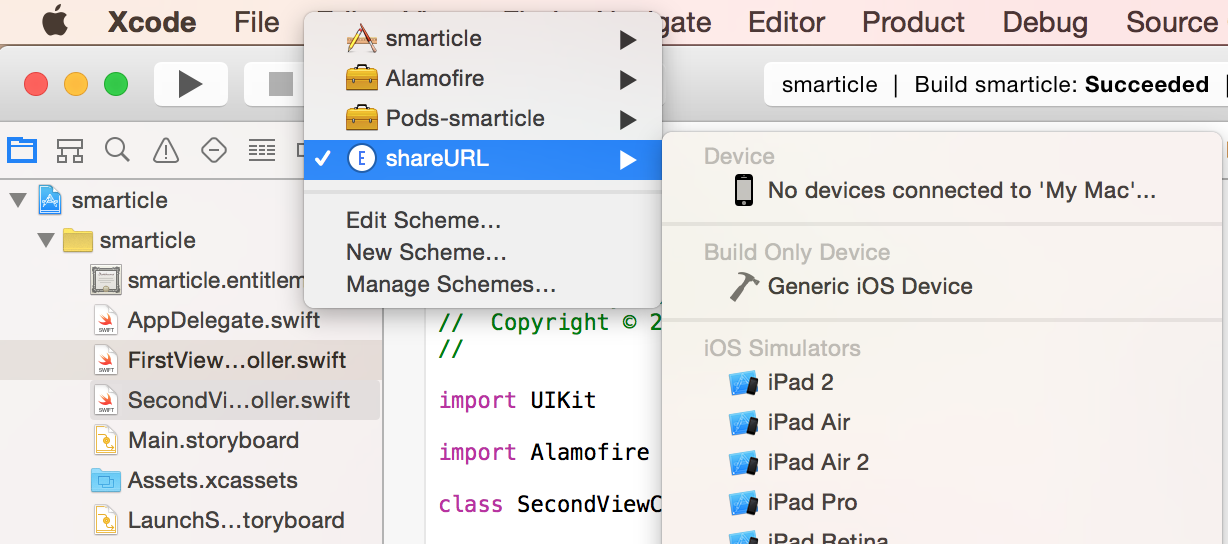
\includegraphics[scale=0.5]{8.jpg}
\end{center}   

Then, hit the "Play" button.  You will be prompted with the following options list.  Choose "Safari" and hit "Run".  

\begin{center}
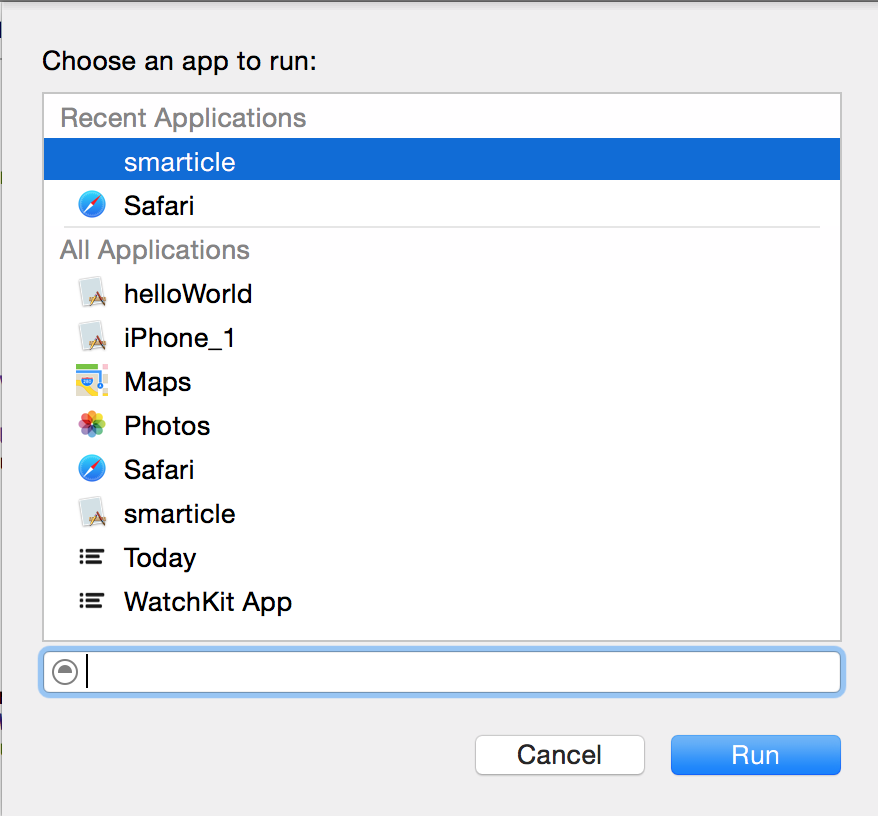
\includegraphics[scale=0.5]{9.jpg}
\end{center}   

Using Safari, find an article that you want to summarize.  Then, hit the "Share" button at the bottom of the screen.  Scroll through the top row until you find "shareURL", and click on it.   
  

\begin{center}
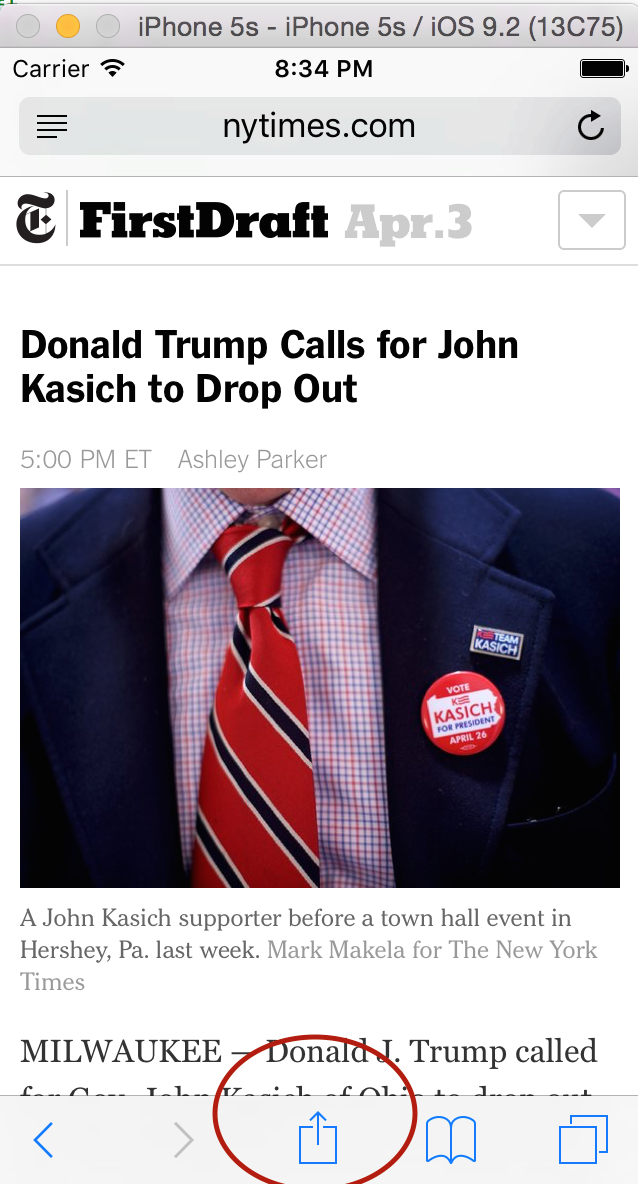
\includegraphics[scale=0.5]{10.jpg}
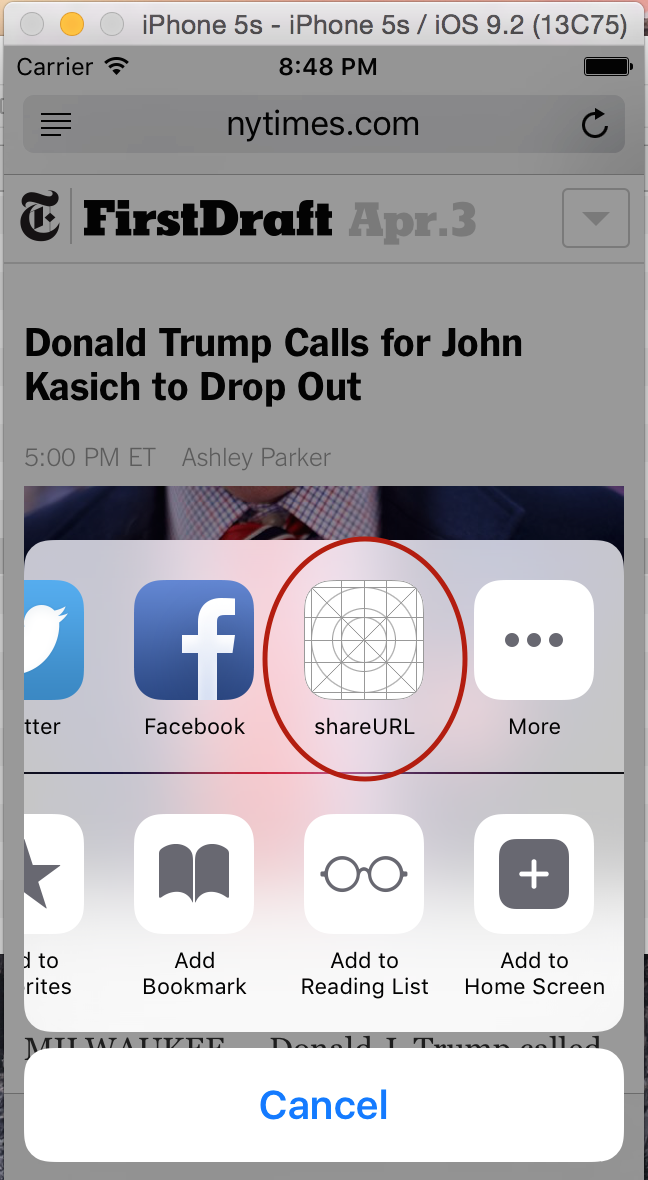
\includegraphics[scale=0.5]{11.jpg}
\end{center}

You will be prompted with the following screen.  Hit "Post" to post the URL of the article to clipboard.

\begin{center}

\includegraphics[scale=0.7]{12.jpg}
\end{center}

\newpage 

Now, hit the home button on the simulator.  This is equivalent to pressing the keyboard shortcut "Command-Shift-H".  Launch the sm@rticle app and paste the URL in the textbox of "Search".  Next, hit "Generate Summary!" to get the summary of your desired article.    

\begin{center}
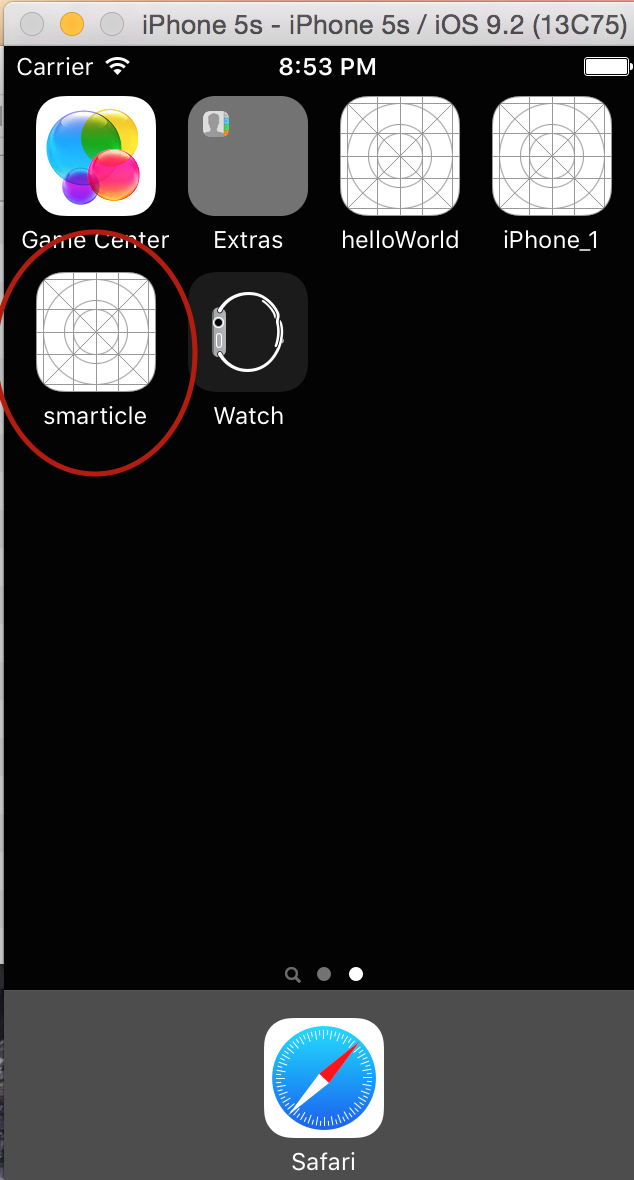
\includegraphics[scale=0.5]{13.jpg}
\end{center}

\newpage
\section{Solution Explained}

\subsection{FirstViewController}
FirstViewController.swift contains the code for the "Search" tab.  A good chunk of this code is dedicated towards implementing the PageRank-based machine learning algorithm for constructing the summary.  I used this research paper (\url{https://web.eecs.umich.edu~mihalcea/papers/mihalcea.emnlp04.pdf}) as the main source of ideas for the algorithm.  See Section 3.3 - Theory Behind the ML Algorithm for more information on what I did.  

The rest of the code is dedicated towards processing/displaying the text of a news article.  First, I used CocoaPods to integrate an open sourced networking library called AlamoFire into my project so that I could perform GET requests.  I could then feed a user-entered URL into the Dandelion API (\url{https://dandelion.eu/}) to extract the source text of the article.  I then cleaned the source text to get the sentences into a format that is friendly for my machine learning algorithm.  Next, the algorithm spits out a ranking of sentences according to how well they represent the content of the article.  The top four sentences are chosen as a summary and printed on the screen, along with the original source text.               

\subsection{SecondViewController}
SecondViewController.swift contains the code for the "Browse" tab.  When a user enters some text to be queried, I submit a GET request with AlchemyAPI to return the titles and URLs of articles containing the search term(s).  I then dynamically generate buttons on the screen with the article titles.  I keep a global array of URLs so that when the user selects an article, the corresponding URL is fed into FirstViewController.  The user can then generate a summary/view the original text of  the article.  

\subsection{Theory Behind the ML Algorithm}
The algorithm I implemented for determining the best sentences to represent the article is based on Google's PageRank, which uses a very similar, unsupervised concept.  We can picture the article as a weighted complete graph, with each sentence being a vertex and edges between every pair of vertices.  The initial weight of a vertex is not important, so we standardize them all to be equal.  However, the final weight of a vertex will tell us how well the corresponding sentence represents the ideas of the article.
The edges also have weights.  The weight $w_e$ of an edge $e = (u, v)$ is determined by a similarity function on the two corresponding vertices (or sentences) $u$, $v$.  Let $S$ be the set of words that are in sentence $u$ and sentence $v$.  Let sentence $u$ have length $n_u$ words and sentence $v$ have $n_v$ words.  I then simply defined $w_e$ (aka the similarity between $u$ and $v$) as
\begin{align*}
w_e = \frac{\card{S}}{\log{n_u} + \log{n_v}}
\end{align*}
Note that this does not have to be the similarity function.  I also tried using other similarity functions that were suggested by the research paper, such as cosine similarity and longest common subsequence.  Nevertheless, upon conducting a brief experiment on 50 articles with these three types of similarity functions, I found that the one I mentioned above seemed to generate the best summaries.  I stored the similarities between each pair of edges in a matrix.  I then used another function to calculate how representative each sentence was of the article by how significant that sentence's edge weights were in comparison to other sentences' edge weights.  This function is displayed below.  For a vertex $v_i$, let $w(v_i)$ denote its weight in the current iteration of the algorithm and let $w'(v_i)$ denote its weight in the previous iteration of the algorithm.  Let $d$ be a damping factor used to speed up convergence.  We then have 
\begin{align*}
w(v_i) = (1 - d) + d \cdot \sum_{j} \frac{w_{e = (v_i, v_j)}}{\sum_{k} w_{e = (v_j, v_k)}} \cdot w'(v_j)  
\end{align*}

I repeatedly applied this function to the vertices weights' until the weights converged on values that were within a 0.001 precision of the weights of the previous iteration.  The vertices/sentences with the top four weights were then selected to summarize the article. 
The intuition behind the algorithm is, as follows: Sentences that end up having high weights share a significant percentage of words with many other sentences.  Thus, it is likely that these highly weighted sentences are the best representation of the content of most of the sentences in the article.  Hence, they make a good summary.  This is the key concept behind the sm@rticle software.              


\end{document}